\documentclass[%
fontsize=12%
,a5paper%
,DIV=15%
]{scrartcl}
%scrartcl



\usepackage{gredocument}
\usepackage{adaptateur}
\usepackage{psaume}

\title{\centrer{Veillée pascale}}
\author{la nuit de la Résurrection}
\date{avec baptêmes d'adultes}

\makeindex
        \definecolor{rubrum}{rgb}{.6,0,0}
        \def\rubrum{\color{rubrum}}%%%%%%%mettre"\def\rubrum{\color{rubrum}}" pour avoir le texte adéquat en rouge
        \def\nigra{\color{black}}
            \redlines
            \definecolor{gregoriocolor}{rgb}{.6,0,0}
        %
        %\let\red\rubrum
        \newcommand{\rep}[2]{\versio{\R \textbf{#1}}{\R \textbf{#2}}}
        \newcommand{\vers}[2]{\versio{\V {#1}}{\V {#2}}}



\begin{document}


\maketitle
\newpage
        \newfontfamily\lettrines[Scale=1.3]{LettrinesPro800}
            \def\gretextformat#1{{\fontsize{\taillepolice}{\taillepolice}\selectfont #1}}
            \def\greinitialformat#1{{\lettrines #1}}
%%%%%%%%%%%%%%%%%%%%%%%%%%%%%%%%%%%%
\titre{Bénédiction du feu et du cierge}
\vspace{0.5cm}
\rubrica{Le Christ, "lumière du monde" (Jn,8,12) va illuminer tout homme cette nuit en sortant du tombeau, il va dissiper les ténèbres du péché}
\rubrica{Le prête bénit le feu, puis trace sur le cierge la croix, l'alpha et l'oméga, et les chiffres de l'année}
\begin{center}
\versio{Christus Heri et hodie}{Le Christ hier et aujourd'hui}
\versio{Princ\'ipium et Finis}{Commencement et Fin}
\versio{Alpha et Omega}{Alpha et Omega}
\versio{Ips\'ius sunt témpora et s\'æcula}{A lui sont les temps et les siècles}
\versio{Ipsi glória et impérium}{A Lui gloire et domination}
\versio{per univérsa aeternit\'atis s\'æcula. Amen}{pendant tous les siècles de l'éternité. Amen}
\end{center}

\titre{Procession du cierge pascal}
\rubrica{Par trois fois le prêtre annonce la lumière qui jaillit, nous répondons pour manifester notre foi en Dieu, Père, Fils et Saint-Esprit}
\versio{Lumen Christi !}{Lumière du Christ !}
\versio{\textbf{Deo Gratias !}}{\textbf{Nous rendons grâce à Dieu !}}

\rubrica{Alors la Lumière se répand par étape à travers toute l'église en allumant nos cierges au cierge bénit}

\titre{Exsultet}
\rubrica{Alors le prêtre chante l'\emph{Exsultet}, chant de gloire et d'honneur à Jésus, Roi éternel, Lumière du monde, et Vainqueur des ténèbres.}
Qu'elle bondisse de joie, la multitude
des \emph{Anges} dans le ciel!
Qu'ils exultent, ces serviteurs de Dieu !
Et pour la victoire d'un si grand Roi,
que retentisse la trompette sacrée !

Que se réjouisse aussi \emph{la terre},
irradiée de si vives clartés : qu'illuminée par la splendeur du Roi éternel,
elle se sente dégagée des ténèbres
qui couvraient l'univers!

Que se réjouisse aussi notre mère
\emph{l'Eglise}, parée des rayons d'une telle
lumière! Et que cette enceinte résonne
sous les voix puissantes des fidèles!

\cantus{Autre}{PerOmnia-ferial}{}{}

Il est vraiment juste et nécessaire
de faire servir nos voix à célébrer,
de toute l'affection du coeur et de
l'âme, le Dieu invisible, Père toutpuissant,
et son Fils unique notre Seigneur Jésus·Christ, qui a payé d'Adam, et effacé de son sang précieux l'arrêt de l'antique péché.(...)

O admirable grandeur de votre tendresse envers nous! O faveur inestimable de votre
amour : pour délivrer l'esclave, vous livrez le Fils !
O péché d'Adam qui devait se commettre pour être effacé par la mort du Christ!
\emph{O heureuse faute qui nous a valu d'avoir un tel, un si grand Rédempteur !}


\titre{Les Lectures}

\rubrica{Nous nous rappelons différents passages de l'Ancien Testament figure du Nouveau}
\begin{enumerate}
\item{La Création, symbole de notre régénération dans le Christ}
\item{Le passage de la Mer Rouge, symbole de notre purification par le passage des eaux du Baptême dans lesquelles sont ensevelis tous nos péchés}
\item{Les promesses rapportées par Isaïe, adressées au nouveau peuple élu}
\item{Les recommandations que Moïse adresse à tous ceux qui feront ou renouvelleront les promesses de leur Baptême}
\end{enumerate}


\titre{Litanies des Saints}
\rubrica{Avant la bénédiction de l'eau baptismale, et les baptêmes, invoquons tous nos aînés dans la Foi qui nous montrent l'exemple}
%Définitions locales

\newcommand{\reponse}[1]{ \hspace*{\stretch{1}} \mbox{\scriptsize #1}}

\newcommand{\miserere}{\reponse{mise\pr{rére}.}}

\newcommand{\ora}{\reponse{o\pr{ra}.}}

\newcommand{\orate}{\reponse{orá\pr{te}.}}

\newcommand{\parce}{\reponse{parce nobis, Dómine.}}

\newcommand{\exaudi}{\reponse{exaudi nos, Dómine.}}

\newcommand{\libera}{\reponse{líbera.}}

\newcommand{\terogamus}{\reponse{te rogámus.}}

\newcommand{\mora}{{~\textbf{'}}}


%Début des litanies

\traduction{%
Seigneur, ayez pitié de nous.
Christ, ayez pitié de nous.
Seigneur, ayez pitié de nous.
Christ, écoutez-nous.
Christ, exaucez-nous.
Père céleste, qui êtes Dieu, ayez pitié de nous.}
\partition{litanies}{kyrie}{}
\medskip


\traduire{%
Fili Redémptor mundi \ac{De}us, \miserere}{%
Fils, Rédempteur du monde, qui êtes Dieu, ayez pitié de nous.}

\traduire{%
Spíritus Sancte \ac{De}us, \miserere}{%
Esprit Saint, qui êtes Dieu,}

\traduire{%
Sancta Trínitas unus \ac{De}us, \miserere}{%
Trinité Sainte, qui êtes un seul Dieu,}

\traduire{%
Sancta Ma\ac{rí}a, \reponse{\normalsize o\pr{ra pro} \ac{no}bis.}}{%
Sainte Marie, priez pour nous.}

\traduire{%
Sancta Dei \ac{Gé}netrix, \ora}{%
Sainte Mère de Dieu,}

\traduire{%
Sancta Virgo \ac{vír}ginum, \ora}{%
Sainte Vierge des vierges,}

\traduire{%
Sancte \ac{Mí}chaël, \ora}{%
Saint Michel,}

\traduire{%
Sancte \ac{Gá}briel, \ora}{%
Saint Gabriel,}

\traduire{%
Sancte \ac{Rá}phaël, \ora}{%
Saint Raphaël,}

\traduire{%
Omnes sancti An\-ge\-li, et Ar\-ch\ac{\-án}ge\-li, \reponse{\normalsize ora\pr{te pro} \ac{no}bis.}}{%
Tous les saints Anges et Archanges,}

\traduire{%
Omnes sancti beatórum Spirítuum \ac{ór}dines,\orate}{%
Tous les ch\oe urs saints des esprits bienheureux,}

\traduire{%
Sancte Ioánnes Bap\ac{tís}ta, \ora}{%
Saint Jean-Baptiste,}

\traduire{%
Sancte \ac{Io}seph, \ora}{%
Saint Joseph,}

\traduire{%
Omnes sancti Patriárch\ae , et Pro\ac{\-phé}\-t\ae , \orate}{%
Tous les saints Patriarches et Prophètes,}

\traduire{%
Sancte \ac{Pe}tre, \ora}{%
Saint Pierre,}

\traduire{%
Sancte \ac{Pau}le, \ora}{%
Saint Paul,}

\traduire{%
Sancte An\ac{dré}a, \ora}{%
Saint André,}

\traduire{%
Sancte Ia\ac{có}be, \ora}{%
Saint Jacques,}

\traduire{%
Sancte Io\ac{án}nes, \ora}{%
Saint Jean,}

\traduire{%
Sancte \ac{Tho}ma, \ora}{%
Saint Thomas,}

\traduire{%
Sancte Ia\ac{có}be, \ora}{%
Saint Jacques,}

\traduire{%
Sancte Phi\ac{líp}pe, \ora}{%
Saint Philippe,}

\traduire{%
Sancte Bartholo\ac{m\'\ae}e, \ora}{%
Saint Barthélémy,}

\traduire{%
Sancte Mat\ac{th\'\ae}e, \ora}{%
Saint Matthieu,}

\traduire{%
Sancte \ac{Si}mon, \ora}{%
Saint Simon,}

\traduire{%
Sancte Thad\ac{d\'\ae}e, \ora}{%
Saint Thaddée,}

\traduire{%
Sancte Mat\ac{thí}a, \ora}{%
Saint Matthias,}

\traduire{%
Sancte \ac{Bár}naba, \ora}{%
Saint Barnabé,}

\traduire{%
Sancte \ac{Lu}ca, \ora}{%
Saint Luc,}

\traduire{%
Sancte \ac{Mar}ce, \ora}{%
Saint Marc,}
\traduire{%
Omnes sancti Apóstoli, et E\-van\-ge\ac{\-lí}\-st\ae ,\orate}{%
Tous les saints Apôtres et Évangélistes,}
\traduire{%
Omnes sancti Discípuli \ac{Dó}mini, \orate}{%
Tous les saints Disciples du Seigneur,}
\traduire{%
Omnes sancti Inno\ac{cén}tes, \orate}{%
Tous les saints Innocents,}
\traduire{%
Sancte \ac{Sté}phane, \ora}{%
Saint Étienne,}
\traduire{%
Sancte Lau\ac{rén}ti, \ora}{%
Saint Laurent,}

\traduire{%
Sancte Vin\ac{cén}ti, \ora}{%
Saint Vincent,}

\traduire{%
Sancti Fabiáne et Sebasti\ac{á}ne, \orate}{%
Saint Fabien et saint Sébastien,}

\traduire{%
Sancti Ioánnes et \ac{Pau}le, \orate}{%
Saint Jean et saint Paul,}

\traduire{%
Sancti Cosma et Dami\ac{á}ne, \orate}{%
Saint Côme et saint Damien,}

\traduire{%
Sancti Gervási et Pro\ac{tá}si, \orate}{%
Saint Gervais et saint Protais,}

\traduire{%
Omnes sancti \ac{Már}tyres, \orate}{%
Tous les saints Martyrs,}

\traduire{%
Sancte Sil\ac{vé}ster, \ora}{%
Saint Silvestre,}

\traduire{%
Sancte Gre\ac{gó}ri, \ora}{%
Saint Grégoire,}

\traduire{%
Sancte Am\ac{bró}si, \ora}{%
Saint Ambroise,}

\traduire{%
Sancte Augu\ac{stí}ne, \ora}{%
Saint Augustin,}

\traduire{%
Sancte Hie\ac{ró}nyme, \ora}{%
Saint Jérôme,}

\traduire{%
Sancte Mar\ac{tí}ne, \ora}{%
Saint Martin,}

\traduire{%
Sancte Nico\ac{lá}e, \ora}{%
Saint Nicolas,}

\traduire{%
Omnes sancti Pontífices, et Confes\ac{só}res, \orate}{%
Tous les saints Pontifes et Confesseurs,}
\traduire{%
Omnes sancti Do\ac{ctó}res, \orate}{%
Tous les saints Docteurs,}

\traduire{%
Sancte An\ac{tó}ni, \ora}{%
Saint Antoine,}

\traduire{%
Sancte Bene\ac{dí}cte, \ora}{%
Saint Benoît,}

\traduire{%
Sancte Ber\ac{nár}de, \ora}{%
Saint Bernard,}

\traduire{%
Sancte Do\ac{mí}nice, \ora}{%
Saint Dominique,}

\traduire{%
Sancte Fran\ac{cí}sce, \ora}{%
Saint Fran\c cois,}

\traduire{%
Omnes sancti Sacerdótes, et Le\ac{\-ví}\-t\ae , }{%
Tous les saints Prêtres et Lévites,}

\traduire{%
Omnes sancti Mónachi, et Ere\ac{mí}t\ae , \orate}{%
Tous les saints Moines et Ermites,}

\traduire{%
Sancta María Magda\ac{lé}na, \ora}{%
Sainte Marie-Madeleine,}

\traduire{%
Sancta \ac{A}gatha, \ora}{%
Sainte Agathe,}

\traduire{%
Sancta \ac{Lú}cia, \ora}{%
Sainte Lucie,}

\traduire{%
Sancta \ac{A}gnes, \ora}{%
Sainte Agnès,}

\traduire{%
Sancta C\ae \ac{cí}lia, \ora}{%
Sainte Cécile,}

\traduire{%
Sancta Catha\ac{rí}na, \ora}{%
Sainte Catherine,}

\traduire{%
Sancta Ana\ac{stá}sia, \ora}{%
Sainte Anastasie,}

\traduire{%
\mbox{Omnes} sanct\ae\ Vírgines et \ac{Ví}du\ae , \orate}{%
Toutes les saintes Vierges et Veuves,}

\traduire{%
Omnes Sancti et Sanct\ae\ \ac{De}i,\hspace*{\stretch{1}} intercedí\pr{te pro} \ac{no}bis.}{%
Tous les Saints et Saintes de Dieu,}




\titre{Bénédiction de l'eau baptismale}
\rubrica{Le prêtre chante une oraison puis une préface sur l'eau}
O Dieu, dont l'Esprit, à l'origine du
monde, planait sur les eaux, pour
leur donner déjà le pouvoir de nous
sanctifier. O Dieu, qui en lavant
par l'eau les crimes d'un monde coupable, avez donné, dans l'inondation
même du déluge, une image de la
régénération, alors que dans le mystère d'un seul et même élément se voyaient tout ensemble et la. ruine
du vice et le principe de la vertu.
Regardez, Seigneur, la face de votre
Eglise et multipliez en elle vos régénération

\rubrica{Le célébrant, de la main étendue, divise l'eau en forme de croix. Ainsi
Dieu en créant le monde avait séparé les eaux d'en-haut de celles d'en bas}
Qu'il vienne, par la secrète union
de sa divinité, féconder cette
eau préparée pour la régénération des hommes

\rubrica{Il touche l'eau avec la main. Le Christ, en touchant l'eau du Jourdain,
lui a enlevé toute puissance nocive; elle est devenue le signe et l'instrument
de notre délivrance.}
Que cette eau soit
une source de vie, une eau qui
régénère, une onde purifiante, afin
que tous ceux qui seront lavés dans
ce bain salutaire, reçoivent, par l'opération du Saint-Esprit qui agira en
eux, la grâce d'une entière purification.

\rubrica{Il fait trois signes de croix sur l'eau, en disant:}
Je te bénis donc, eau créée, par
le Dieu \x vivant, par le Dieu
vrai, par le Dieu \x saint : par \x 
le Dieu, dont la parole te sépara de
la terre à l'origine et dont l'Esprit planait sur toi.

\rubrica{Ici, il divise l'eau avec la main et en jette vers les quatre parties du monde,
Ce geste rappelle le fleuve qui, sorti de l' Eden, se divisait en quatre branches,
pour arroser « la terre entière »}

\rubrica{Il plonge ensuite trois fois le cierge dans l'eau, pour rappeler que le Christ
a sanctifié les eaux en descendant dans le Jourdain et que la Sainte Trinité
s'est manifestée à ce moment; il chante à chaque fois}
Que la vertu du Saint-Esprit
descende sur toute l'eau de cette fontaine.

\rubrica{Puis le prêtre extrait de l'eau qui servira tout le temps pascal, et termine la consécration de l'eau par l'infusion des Huiles consacrées le Jeudi Saint par l'évêque}

\versio{Sanctificétur et fecundétur
fons iste Oleo sal\'utis renascéntibus ex eo, in vitam aetérnam.}
{Que cette fontaine soit sanctifiée et fécondée par l'Huile du salut pour ceux qui y renaîtront à la vie éternelle.}
\rep{Amen.}{Ainsi soit-il.}

\versio{
Infusio Chrismatis D\'omini 
nostri Jesu Christi, et Spiritus 
Sancti Paracliti, fiat in n\'omine 
sanctae Trinit\'atis.}
{Que l'infusion du Chrême de notre Seigneur Jésus-Christ et de l'Esprit-Saint Consolateur, se fasse au nom de la sainte Trinité.}
\rep{Amen.}{Ainsi soit-il.}

\versio{
Commixtio Chrismatis sanctificati\'onis, et Olei uncti\'nis, et aquae bapt\'ismatis, p\'ariter fiat in n\'omine Pa\x tris, et
Fi\x lii, et Spiritus \x~ Sancti.}{
Que le mélange du Chrême sanctifiant, de l'Huile d'onction et
de l'eau baptismale s'opère également
au nom du Père, \x~ et du Fils, \x~ et
du Saint \x~ Esprit. }
\rep{Amen.}{Ainsi soit-il.}

\titre{Le Sacrement de Baptême}
\rubrica{Le prêtre administre alors le sacrement de Baptême aux catéchumènes}
\textsc{Le célébrant :} - Croyez-vous en Dieu, le Père tout-puissant,
Créateur du ciel et de la terre?

\textsc{Le catéchumène :} - J'y crois.

- Croyez-vous en Jésus-Christ, son Fils unique, notre
Seigneur, qui est né et quui est mort pour nous

- J'y crois.

- Croyez-vous au Saint-Esprit, à la Sainte Église
catholique, à la communion des Saints, à la rémission
des péchés, à la résurrection de la chair et à la vie
éternelle?

- J'y crois.

- Voulez-vous être baptisé ?

- Je le veux.

\rubrica{Le célébrant verse de l'eau baptismale par trois fois sur la tête de celui qui
doit êre baptisé, en disant en latin :}
\textsc{\rubrum{N.},\nigra{} JE VOUS BAPTISE AU NOM DU PÈRE, ET DU FILS, ET DU SAINT ESPRIT.}

\titre{Renouvellement des promesses du baptême}
\rubrica{Alors, tous nous sommes invités à renouveler la promesse de fidélité à Dieu.}

\titre{Deuxième partie des litanies}
\rubrica{On termine alors les litanies, en demandant la protection divine ; pendant ce temps, le chœur est préparé pour la messe de la Résurrection}

\traduction{%
Soyez-nous propice, pardonnez-nous, Seigneur.}
\partition{litanies}{propitius}{}
\medskip


\traduire{%
\parbox{\linewidth}{Propí\pr{tius}\ac{ es}to,\\ \hspace*{\stretch{1}} \mbox{exáudi nos, Dómine.}}}{%
\parbox{\linewidth}{Soyez-nous propice,\\ \hspace*{\stretch{1}} \mbox{exaucez-nous, Seigneur.}}}

\traduire{%
Ab \pr{omni}\ac{ ma}lo,\\ \hspace*{\stretch{1}} \mbox{líbera nos, Dómine.}}{%
De tout mal, délivrez-nous, Seigneur.}

\traduire{%
Ab o\pr{mni pec}\ac{cá}to, \libera}{%
De tout péché,}

\traduire{%
Ab \pr{ira}\ac{ tu}a, \libera}{%
De votre col\`ere,}

\traduire{%
A subitánea et impro\pr{vísa}\ac{ mor}te, \libera}{%
De la mort subite et imprévue,}

\traduire{%
Ab insídi\pr{is di}\ac{á}boli, \libera}{%
Des embûches du démon,}

\traduire{%
Ab ira, et ódio, et omni mala \pr{volun}\ac{tá}te, \libera}{%
De la colère, de la haine et de toute malveillance,}

\traduire{%
A spíritu forni\pr{cati}\ac{ó}nis, \libera}{%
De l'esprit d'impureté,}

\traduire{%
A fúlgure et \pr{tempe}\ac{stá}te, \libera}{%
De la foudre et de la tempête,}

\traduire{%
A flagéllo \pr{terr\ae}\ac{mó}tus, \libera}{%
Du fléau des tremblements de terre,}

\traduire{%
A peste, fa\pr{me, et}\ac{ bel}lo, \libera}{%
De la peste, de la famine et de la guerre,}

\ifthenelse{\equal{\commandkey{quaranteheures}}{oui}}{%
\traduire{%
Ab imminénti\pr{bus per}\ac{í}culis, \libera}{%
Des périls imminents,}%
}{}

\traduire{%
A mor\pr{te per}\ac{pé}tua, \libera}{%
De la mort éternelle,}

\traduire{%
Per mystérium sanct\ae\ Incarnati\pr{ónis}\ac{ tu}\ae , \libera}{%
Par le mystère de votre sainte Incarnation,}

\traduire{%
Per Ad\pr{véntum}\ac{ tu}um, \libera}{%
Par votre avènement,}

\traduire{%
Per Nativi\pr{tátem}\ac{ tu}am, \libera}{%
Par votre naissance,}

\traduire{%
Per Baptísmum, et sanctum Ieiú\pr{nium}\ac{ tu}um, \libera}{%
Par votre baptême et votre saint jeûne,}

\traduire{%
Per Crucem, et Passi\pr{ónem}\ac{ tu}am, \libera}{%
Par votre croix et votre Passion,}

\traduire{%
Per Mortem, et Sepul\pr{túram}\ac{ tu}am, \libera}{%
Par votre mort et votre sépulture,}

\traduire{%
Per sanctam Resurrecti\pr{ónem}\ac{ tu}am, \libera}{%
Par votre sainte Résurrection,}

\traduire{%
\parbox[t]{\linewidth}{Per admirábilem Ascensi\pr{ónem}\ac{ tu}am, \libera}}{%
Par votre admirable Ascension,}

\traduire{%
Per advéntum Spíritus San\pr{cti pa}\ac{\-rá}\-cli\-ti, \libera}{%
Par l'avènement du Saint Esprit consolateur,}

\traduire{%
In di\pr{e iu}\ac{dí}cii, \libera}{%
Au jour du jugement,}


\traduction{%
Pécheurs, nous vous prions, exaucez-nous.}
\partition{litanies}{peccatores}{}
\medskip


\traduire{%
Ut no\pr{bis}\ac{ par}cas,\terogamus}{%
Daignez nous pardonner,}

\traduire{%
Ut nobis \pr{in}\ac{dúl}geas,\terogamus}{%
Daignez nous faire grâce,}

\traduire{%
Ut ad veram p\ae niténtiam nos perdúcere \pr{di}\ac{gné}ris,\terogamus}{%
Daignez nous conduire à une véritable pénitence,}

\traduire{%
Ut Ecclésiam tuam sanctam\mora\ régere, et conserváre \pr{di}\ac{gné}ris,\terogamus}{%
Daignez gouverner et conserver votre Église sainte,}

\traduire{%
Ut Domnum apostólicum, et omnes ecclesiásticos órdines\mora\  in sancta religióne conserváre \pr{di}\ac{gné}ris, \terogamus}{%
Daignez maintenir dans votre sainte religion le souverain Pontife et tous les ordres de la hiérarchie ecclésiastique,}

\traduire{%
Ut inimícos sanct\ae\ Ecclési\ae\mora\ humiliáre \pr{di}\ac{gne}ris,\terogamus}{%
Daignez humilier les ennemis de la sainte Église,}

\traduire{%
\mbox{Ut Régibus, et Princípibus} christiánis\mora\ pacem, et veram concórdiam donáre \pr{di}\ac{gné}ris,\terogamus}{%
Daignez donner aux Rois et Princes chrétiens la paix et une vraie concorde,}

\traduire{%
Ut cuncto pópulo christiáno\mora\ pacem et unitátem largíri \pr{di}\ac{gné}ris,\terogamus}{%
Daignez accorder à tout le peuple chrétien la paix et l'unité,}

\traduire{%
Ut omnes errántes ad unitátem Ecclési\ae\ revocáre,\mora\ et infidéles univérsos ad Evangélii lumen perdúcere \pr{di}\ac{gné}ris,\terogamus}{%
Daignez rappeler tous les égarés à l'unité de l'Église, et amener tous les infidèles à la lumièere de l'Évangile,}

\traduire{%
\parbox[t]{\linewidth}{Ut nosmetípsos in tuo sancto servítio\mora\ confortáre, et conserváre \pr{di}\ac{gné}ris,\terogamus}}{%
\parbox[t]{\linewidth}{Daignez nous fortifier et nous conserver dans votre saint service,}}

\traduire{%
\parbox[t]{\linewidth}{Ut mentes nostras\mora\ ad c\ae léstia desidéri\pr{a}\ac{ é}rigas,\terogamus}}{%
\parbox[t]{\linewidth}{Daignez élever nos esprits aux célestes désirs,}}

\traduire{%
Ut ómnibus benefactóribus nostris\mora\ sempitérna bona \pr{re}\ac{trí}buas,\terogamus}{%
Daignez récompenser tous nos biensfaiteurs par les biens éternels,}

\traduire{%
Ut ánimas nostras,\mora\ fratrum, propinquórum et benefactórum nostrórum ab \ae térna damnatióne \pr{e}\ac{rí}pias,\terogamus}{%
Daignez préserver de l'éternelle damnation nos âmes, celles de nos frères, de nos proches et de nos bienfaiteurs,}

\traduire{%
Ut fructus terr\ae\mora\ dare, et conserváre \pr{di}\ac{gné}ris,\terogamus}{%
Daignez nous donner et nous conserver les biens de la terre,}

\traduire{%
Ut ómnibus fidélibus defúnctis\mora\ réquiem \ae térnam donáre \pr{di}\ac{gné}ris, \terogamus }{%
Daignez donner à tous les fidèles défunts le repos éternel,}

\ifthenelse{\equal{\commandkey{ordinations}}{oui}}{%
%
\rubrique{L'évêque se lève pour bénir les Ordinands :}
\traduire{%
Ut hos eléctos bene{\x}dícere \pr{di}\ac{gné}ris,\terogamus}{%
Daignez bé\x{}nir ces élus,}

\traduire{%
Ut hos eléctos bene{\x}dícere et sancti{\x}ficáre \pr{di}\ac{gné}ris, \terogamus}{%
Daignez bé\x{}nir et sancti\x{}fier ces élus,}

\traduire{%
Ut hos eléctos bene{\x}\-dícere, sancti{\x}\-ficáre et conse{\x}\-cráre  \pr{di}\ac{gné}ris, \terogamus}{%
Daignez bé\x{}nir, sancti\x{}fier et consa\x{}crer ces élus,}

\rubrique{L'évêque s'agenouille de nouveau tandis que les chantres achèvent les litanies :}
%
}{}

\traduire{%
Ut nos exaudíre \pr{di}\ac{gné}ris,\terogamus}{%
Daignez nous exaucer,}

\traduire{%
Fi\pr{li}\ac{ De}i,\terogamus}{%
Fils de Dieu,}


\traduction{%
Agneau de Dieu, qui effacez les péchés du monde, pardonnez-nous, Seigneur.
Agneau de Dieu, qui effacez les péchés du monde, exaucez-nous, Seigneur.
Agneau de Dieu, qui effacez les péchés du monde, ayez pitié de nous.
Christ, écoutez-nous.
Christ, exaucez-nous.
Seigneur, ayez pitié de nous !
Christ, ayez pitié de nous !
Seigneur, ayez pitié de nous !}
\partition{litanies}{conclusion}{}

\ifthenelse{\equal{\commandkey{quaranteheures}}{oui}%
\OR \equal{\commandkey{rogations}}{oui}}{%
%
\traduction{%
Mon Dieu, venez à mon aide ; Seigneur, hâtez-vous de me secourir !%
}
\partition{PP-Psaumes}{Intonation-069}{}

\traduire{%
\psaume[ton=4g%
,premierverset=2%
,dernierverset=6%
,numero=2%
]{069}
\gloria[ton=4g]%
}{%
\psaume[premierverset=2%
,dernierverset=6%
,numero=2%
]{069-fr}
\gloriafr%
}

\traduire{%
\V.~Salvos fac servos tuos.

\R.~Deus meus, sperántes in te.}{%
\V.~Sauvez vos serviteurs,

\R.~Qui espèrent en vous, mon Dieu.%
}

\traduire{%
\V.~Esto nobis, Dómine, turris fortitúdinis.

\R.~A fácie inimíci.%
}{%
\V.~Soyez-nous, Seigneur, une tour fortifiée.

\R.~En face de l'ennemi.%
}

\traduire{%
\V.~Nihil profíciat inimícus in nobis.

\R.~Et fílius iniquitátis non appónat nocére nobis.%
}{%
\V.~Que l'ennemi n'ait aucune emprise sur nous.

\R.~Et que le fils d'iniquité n'ose point nous nuire.%
}

\traduire{%
\V.~Dómine, non secúndum peccáta nostra fácias nobis.

\R.~Neque secúndum iniquitátes nostras retríbuas nobis.%
}{%
\V.~Seigneur, ne nous traitez pas selon nos fautes.

\R.~Et ne nous châtiez pas selon nos iniquités.%
}

\traduire{%
\V.~Orémus pro Pontífice nostro \emph{N}.

\R.~Dóminus consérvet eum, et vivíficet eum, et beátum fáciat eum in terra, et non tradat eum in ánimam inimicórum eius.%
}{%
\V.~Prions pour notre Pontife \emph{N}.

\R.~Que le Seigneur veille sur lui, lui garde la vie et fasse son bonheur sur terre, empêchant qu'il ne tombe à la merci de ses ennemis.}

\traduire{%
\V.~Orémus pro benefactóribus nostris.

\R.~Retribúere dignáre, Dómine, ómnibus nobis bona faciéntibus propter nomen tuum, vitam ætérnam. Amen.}{%
\V.~Prions pour nos bienfaiteurs.

\R.~Daignez, Seigneur, donner la vie éternelle en récompense à tous ceux qui nous ont fait du bien en l'honneur de votre Nom. \ainsi.}

\traduire{%
\V.~Orémus pro ómnibus fidélibus defúnctis.

\R.~Réquiem ætérnam dona eis, Dómine, et lux perpétua lúceat eis.}{%
\V.~Prions pour tous les fidèles défunts.

\R.~Donnez leur, Seigneur, le repos éternel, et que la lumière sans fin resplendisse à leurs yeux.}

\traduire{%
\V.~Requiéscant in pace.

\R.~Amen.}{%
\V.~Qu'ils reposent en paix.

\R.~\ainsi.}

\traduire{%
\V.~Pro frátribus abséntibus.

\R.~Salvos fac servos tuos, Deus meus, sperántes in te.}{%
\V.~Pour nos frères absents.

\R.~Protégez, mon Dieu, vos serviteurs qui espèrent en vous.}

\traduire{%
\V.~Mitte eis, Dómine, auxílium de sancto.

\R.~Et de Sion tuére eos.}{%
\V.~Envoyez-leur, Seigneur, votre secours de votre sanctuaire.

\R.~Et de Sion, protégez-les.}

\traduire{%
\V.~Dómine, exáudi oratiónem meam.

\R.~Et clamor meus ad te véniat.}{%
\V.~Seigneur, écoutez ma prière.

\R.~Et que mon appel parvienne jusqu'à vous.}
%
}

\ifthenelse{\equal{\commandkey{rogations}}{oui}}{%
\traduire{%
\V.~Dóminus vobíscum.

\R.~Et cum spíritu tuo.}{%
\V.~Le Seigneur soit avec vous.

\R.~Et avec votre esprit.}

\traduire{%
Orémus.}{%
Prions.}

\traduire{%
Deus, cui próprium est miseréri semper et párcere : súscipe deprecatiónem nostram ; ut nos, et omnes fámulos tuos, quos delictórum cátena constríngit, miserátio tuæ pietátis cleménter absólvat.}{%
Ô Dieu, vous à qui il appartient en propre d'avoir pitié et de pardonner, accueillez notre prière : que votre bonté miséricordieuse daigne nous délivrer, ainsi que tous vos serviteurs, qu'entravent les liens du péché.}

\traduire{%
Exáudi, qu\'æsumus, Dómine, súpplicum preces : et confiténtium tibi parce peccátis ; ut páriter nobis indulgéntiam tríbuas benígnus et pacem.}{%
Seigneur, exaucez les prières de ceux qui vous supplient, et pardonnez les péchés de ceux qui les confessent ; que votre bonté nous accorde en même temps le pardon et la paix.}

\traduire{%
Ineffábilem nobis, Dómine, misericórdiam tuam cleménter osténde : ut simul nos et a peccátis ómnibus éxuas ; et a p\oe nis, quas pro his merémur, erípias.}{%
Que votre miséricorde ineffable, Seigneur, se manifeste à vous avec clémence, nous délivrant de tous nos péchés et nous arrachant aux châtiments qu'ils nous ont mérités.}

\traduire{%
Deus, qui culpa offénderis, pæniténtia placáris : preces pópuli tui supplicántis propítius réspice ; et flagélla tuæ iracúndiæ, quæ pro peccátis nostris merémur, avérte.}{%
Ô Dieu, que le péché offense et que la pénitence apaise, regardez avec bonté les prières de votre peuple suppliant, et détournez les fléaux de votre colère, que nous méritons pour nos péchés.}

\traduire{%
Omnípotens sempitérne Deus, miserére fámulo tuo Pontífici nostro \emph{N.} : et dírige eum secúndum tuam cleméntiam in viam salútis ætérnæ ; ut, te donánte, tibi plácita cúpiat, et tota virtúte perfíciat.}{%
Dieu tout-puissant et éternel, ayez pitié de votre serviteur, notre Pontife \emph{N}., et, par votre bonté, conduisez-le dans la voie du salut éternel ; donnez-lui de vouloir ce qui vous est agréable, et de l'accomplir de toutes ses forces.}

\traduire{%
Deus, a quo sancta desidéria, recta consília, et iusta sunt ópera : da servis tuis illam, quam mundus dare non potest, pacem ; ut et corda nostra mandátis tuis dédita, et hóstium subláta formídine, témpora sint tua protectióne tranquílla.}{%
Ô Dieu, de qui viennent les saints désirs, les jugements droits et les \oe uvres justes, donnez à vos serviteurs cette paix que le monde ne peut donner. Que nos c\oe urs soient tout à vos commandements, que s'éloigne de nous la frayeur inspirée par nos ennemis, et que votre protection donne le calme à notre temps.}

\traduire{%
Ure igne Sancti Spíritus renes nostros et cor nostrum, Dómine : ut tibi casto córpore serviámus, et mundo corde placeámus.}{%
Enflammez, Seigneur, du feu du Saint-Esprit nos reins et nos c\oe urs, afin que nous vous servions en un corps chaste, et que nous vous plaisions par un c\oe ur pur.}

\traduire{%
Fidélium Deus ómnium Cónditor et Redémptor, animábus famulórum famularúmque tuárum remissiónem cunctórum tríbue peccatórum : ut indulgéntiam, quam semper optavérunt, piis supplicatiónibus consequántur.}{%
Créateur et Rédempteur de tous les fidèles, ô Dieu, accordez aux âmes de vos serviteurs et de vos servantes la rémission de tous leurs péchés. Qu'elles obtiennent, par nos humbles supplications, l'indulgence qu'elles ont toujours souhaitée.}

\traduire{%
Actiónes nostras, qu\'æsumus Dómine, aspirándo pr\'æveni, et adiuvándo proséquere : ut cuncta nostra orátio et operátio a te semper incípiat, et per te c\oe pta finiátur.}{%
Prévenez, Seigneur, de votre inspiration nos actions, et accompagnez-les de votre secours : que notre prière et notre activité tout entières commencent toujours par vous, et qu'une fois entreprises, elles soient par vous achevées.}

\traduire{%
Omnípotens sempitérne Deus, qui vivórum domináris simul et mortuórum, omniúmque miseréris, quos tuos fide et ópere futúros esse prænóscis : te súpplices exorámus ; ut pro quibus effúndere preces decrévimus, quosque vel præsens s\'æculum adhuc in carne rétinet, vel futúrum iam exútos córpore suscépit, intercedéntibus ómnibus Sanctis tuis, pietátis tuæ cleméntia, ómnium delictórum suórum véniam consequántur. Per Dóminum nostrum Iesum Christum Fílium tuum : qui tecum vivit et regnat in unitáte Spíritus Sancti Deus, per ómnia s\'æcula sæculórum.}{%
Dieu tout-puissant et éternel, qui êtes maître des vivants comme des morts, et qui faites miséricorde à tous ceux qui seront vôtres par la foi et les \oe uvres, et que vous connaissez dès à présent, nous vous implorons pour ceux à l'intention de qui nous voulons vous adresser nos prières, soit que leur corps les retienne encore dans le siècle présent, soit que, dépouillés de ce corps, ils aient été reçus déjà dans le monde à venir : que l'intercession de tous vos saints leur obtienne de votre bonté clémente le pardon de tous leurs péchés. Par notre Seigneur Jésus-Christ...}

\traduire{%
\R.~Amen.}{%
\R.~\ainsi.}

\traduire{%
\V.~Dóminus vobíscum.

\R.~Et cum spíritu tuo.}{%
\V.~Le Seigneur soit avec vous.

\R.~Et avec votre esprit.}

\traduire{%
\V.~Exáudiat nos omnípotens et miséricors Dóminus.}{%
\V.~Que le Seigneur tout-puissant et miséricordieux nous exauce.}

\traduire{%
\V.~Amen.}{%
\V.~\ainsi.}

\traduire{%
\V.~Et fidélium ánimæ per misericórdiam Dei requiéscant in pace.}{%
\V.~Et que, par la miséricorde de Dieu, les âmes des fidèles défunts reposent en paix.}

\traduire{%
\V.~Amen.}{%
\V.~\ainsi.}
%
}{}


\cleardoublepage
\titre{Messe de la Résurrection}
\rubrica{Après nous avoir fait revivre la grâce de notre baptême, l'Eglise nous invite à offrir avec elle le saint sacrifice de la messe. C'est l'action de grâces, où nous présentons à Dieu l'Agneau pascal, immolé pour le salut du monde}

\titre{Kyrie}
\cantus{Kyriale}{Kyrie-I}{I}{}

\titre{Gloria}
\rubrica{C'est au moment du Gloria que la joie pascale est complète, les cloches sonnent à nouveau, l'orgue se réveille, et toutes les statues quittent leur voile de deuil}
\vulgo{Gloire à Dieu au plus haut des cieux, et paix sur la terre aux hommes de bonne volonté. Nous vous louons, nous vous bénissons, nous vous adorons, nous vous glorifions. Nous vous rendons grâces pour votre gloire immense, Seigneur Dieu, Roi du ciel, Dieu Père tout-puissant. Seigneur Fils unique, Jésus-Christ, Seigneur Dieu, Agneau de Dieu, Fils du Père, vous qui enlevez les péchés du monde, ayez pitié de nous ; vous qui enlevez les péchés du monde, accueillez notre prière ; vous qui siégez à la droite du Père, ayez pitié de nous. Car vous êtes le seul Saint, le seul Seigneur, le seul Très-Haut, Jésus-Christ, avec le Saint-Esprit, dans la gloire de Dieu le Père. Ainsi soit-il.}
\cantus{Kyriale}{Gloria-I}{I}{}

\titre{Oraison}
Ô Dieu, qui illuminez cette très sainte nuit de la gloire de la résurrection du Seigneur, conservez dans les nouveaux enfants de votre famille l’esprit d’adoption que vous leur avez donné ; afin que, renouvelés de corps et d’esprit, ils vous servent dans l’innocence. Par le même Jésus-Christ Notre-Seigneur.

\titre{Epître}
\rubrica{Saint Paul nous invite à vivre et à renouveller la grâce de Dieu en nous : vivons en ressuscités.}

\titre{Alleluia}
\rubrica{Unissons-nous avec le prêtre, en reprenant l'Alleluia}
\cantus{Alleluia}{Confitemini_Quoniam_SabbatoSancto_jubilus}{VIII}{}
Célébrez le Seigneur, parce qu’il est bon, parce que sa miséricorde est éternelle.

Nations, louez toutes le Seigneur ; peuples, louez-le tous. Car sa miséricorde a été affermie sur nous, et la vérité du Seigneur demeure éternellement.

\titre{Evangile}
\nopagebreak
\rubrica{Récit de la découverte de la Résurrection}

\titre{Offertoire}
\rubrica{À l'Offertoire l'Église offre le Corps et le Sang du Christ, représentés par le pain et le vin. Notre Seigneur a communiqué à son Église le pouvoir d'offrir le même sacrifice qu'il offrit sur la Croix. L'Église s'y unit comme victime. \emph{Le Christ lui-même est à la fois le prêtre qui offre et la victime qui est offerte. Le sacrifice de l'Église est le sacrement quotidien du sacrifice du Christ. L'Église, qui est le corps dont il est la tête, s'y offre elle-même par lui. C'est pourquoi dans ce sacrement l'Église elle-même est offerte dans ce qu'elle offre.} (S.~Augustin). Nous sommes donc une seule victime avec le Christ, unissant nos propres offrandes et nos sacrifices à celui du Christ et de l'Église.}
Recevez, Père saint, Dieu éternel et tout-puissant, cette offrande sans tache, que moi, votre indigne serviteur, je vous présente, à vous, mon Dieu vivant et vrai, pour mes péchés, offenses et négligences sans nombre, pour tous ceux qui m'entourent, ainsi que pour tous les fidèles vivants et morts : qu'elle serve à mon salut et au leur pour la vie éternelle. Ainsi soit-il.

\rubrica{Le diacre prépare le calice en y versant le vin ; le sous-diacre y ajoute quelques gouttes d'eau que le prêtre bénit (s'il est seul le prêtre accomplit lui-même ces cérémonies). L'eau mêlée au vin figure l'union en Jésus-Christ de la nature humaine à la personne divine, et symbolise aussi le chrétien intimement uni au Christ. Le vin et l'eau rappellent le Sang et l'eau qui coulèrent du côté du Christ percé par la lance. \emph{Quand le vin et l'eau sont mêlés dans le calice, le peuple est uni au Christ et la foule des croyants est associée et réunie à celui en qui elle croit.} (S.~Cyprien)}
Dieu, ✠ qui, d'une manière admirable, avez créé la nature humaine dans sa noblesse, et l'avez restaurée d'une manière plus admirable encore, accordez-nous, selon le mystère de cette eau et de ce vin, de prendre part à la divinité de celui qui a daigné partager notre humanité, Jésus-Christ votre Fils, Notre Seigneur, qui, étant Dieu, vit et règne avec vous en l'unité du Saint-Esprit, dans tous les siècles des siècles. \mbox{Ainsi soit-il}.\looseness=1

\subsection*{Encensement}

\rubrica{Comme l'encens, consumé par le feu, s'élève en vapeur odorante, ainsi l'Église avec le Christ, consumée par le feu du Saint-Esprit, s'élève en sacrifice envers Dieu. On encense les oblats (le pain et le vin), puis l'autel, le prêtre, et enfin le clergé et les fidèles.}

\subsection*{%
Oraison silencieuse (Secrète)%
}
Agréez, nous vous en supplions. Seigneur, les prières de votre peuple avec l’oblation de ces hosties, en sorte qu’empreintes de l’esprit du mystère pascal, elles nous servent, grâce à votre action, de remède pour l’éternité.


\subsection*{%
Préface%
}
\rubrica{Par le chant de la Préface le prêtre rend grâces à Dieu au nom de l'Église pour l'œuvre du salut réalisée par Jésus-Christ.}

\versio{%
℣. Per ómnia sǽcula sæculórum. ℟. Amen.}{%
℣. Dans tous les siècles des siècles. ℟. Ainsi soit-il.}

\versio{%
℣. Dóminus vobíscum.}{%
℣. Le Seigneur soit avec vous.}

\versio{%
℟. Et cum spíritu tuo.}{%
℟. Et avec votre esprit.}

\versio{%
℣. Sursum corda.}{%
℣. Élevons nos cœurs.}

\versio{%
℟. Habémus ad Dóminum.}{%
℟. Ils sont tournés vers le Seigneur.\looseness=-1}

\versio{%
℣. Grátias agámus Dómino Deo nostro.}{%
℣. Rendons grâces au Seigneur notre Dieu.}

\versio{%
℟. Dignum et iustum est.}{%
℟. C'est juste et nécessaire.}

Il est vraiment juste et nécessaire,
c’est notre devoir et c’est notre salut,
de vous louer, Seigneur, en tout temps,
mais surtout avec encore plus de gloire en cette nuit
où le Christ, notre Pâque, a été immolé.
Car il est le véritable Agneau
qui a ôté les péchés du monde.
Il a détruit notre mort par la sienne
et nous a rendu la vie en ressuscitant.
C’est pourquoi, avec les Anges et les Archanges,
avec les Trônes et les Dominations,
et avec toute la milice de l’armée céleste
nous chantons l’hymne de votre gloire
en disant sans cesse :

\subsection*{Sanctus}
\vulgo{Saint, saint, saint le Seigneur, Dieu des armées. Les cieux et la terre sont remplis de votre gloire ; hosanna au plus haut des cieux ! Béni soit celui qui vient au nom du Seigneur ; hosanna au plus haut des cieux !}
\cantus{Kyriale}{Sanctus-I.gabc}{IV}{}

\subsection*{Canon}
\rubrica{Canon signifie règle. Cette partie de la messe est une règle intangible. Les prières du Canon remontent au-delà du VI\ieme{} siècle, voire pour certaines à l'Apôtre Pierre lui-même.}

\rubrica{À cet instant commence le rite consécratoire proprement dit. Il convient de se tenir à genoux. Le prêtre étend les mains sur le pain et le vin, comme faisait le Grand Prêtre de l'Ancien Testament sur la victime que l'on immolait pour l'expiation des péchés. Jésus-Christ a pris sur lui nos péchés pour les expier.}

Ainsi donc, Seigneur, ce sacrifice que nous vous offrons et, avec tous vos enfants, aujourd’hui spécialement pour ceux que vous avez daigné régénérer par l’eau et l’Esprit-Saint en leur accordant la rémission de tous leurs péchés, acceptez-le avec bienveillance ; disposez dans votre paix les jours de notre vie ; veuillez nous arracher à l'éternelle damnation et nous compter au nombre de vos élus. Par le Christ notre Seigneur. Ainsi \mbox{soit-il}.

\rubrica{Le prêtre récite alors l'histoire de l'institution de l'eucharistie en accomplissant les mêmes gestes que le Christ.}

\versio{%
Qui prídie quam paterétur, accépit panem in sanctas ac venerábiles manus suas, et elevátis óculis in cælum ad te Deum Patrem suum omnipoténtem, tibi grátias agens, bene ✠ díxit, fregit, dedítque discípulis suis, dicens : Accípite, et manducáte ex hoc omnes.}{%
Celui-ci, la veille de sa Passion, prit du pain dans ses mains saintes et adorables, et, les yeux levés au ciel vers vous, Dieu, son Père tout-puissant, vous rendant grâces, il ✠ bénit ce pain, le rompit et le donna à ses disciples en disant : Prenez et mangez-en tous.}


\rubrica{Le prêtre prononce alors les paroles mêmes de Notre-Seigneur. Par ces paroles il opère la conversion du pain au saint Corps du Christ.}

\versio{%
\scalebox{.91}[1]{\textsc{\addfontfeatures{Renderer=Basic}Hoc est enim Corpus meum.}}\par%
}{%
\textsc{\addfontfeatures{Renderer=Basic}Car ceci est mon Corps.}\par%
}

%\vspace{1\baselineskip plus 2\baselineskip}

\rubrica{Ces paroles étant prononcées, le prêtre fait la génuflexion pour adorer le saint Corps, l'élève pour le présenter à l'adoration des fidèles, le dépose sur l'autel et fait de nouveau la génuflexion. Le prêtre reprend le récit de l'institution de l'eucharistie :}

\versio{%
Símili modo postquam cenátum est, accípiens et hunc præclárum Cálicem in sanctas ac venerábiles manus suas : item tibi grátias agens, bene ✠ díxit, dedítque discípulis suis, dicens : Accípite, et bíbite ex eo omnes.}{%
De même, après le repas, il prit aussi ce précieux calice dans ses mains saintes et adorables, vous rendit grâces encore, le ✠ bénit et le donna à ses disciples en disant : Prenez et buvez-en tous.}

\rubrica{Prononçant alors les paroles mêmes de Notre-Seigneur, le prêtre opère la conversion du vin au précieux Sang du Christ.}
%
\nopagebreak\smallskip%
%
\versio{%
\textsc{\addfontfeatures{Renderer=Basic}Hic est enim Calix Sánguinis mei, novi et ætérni Testaménti : mystérium fídei : qui pro vobis et pro multis effundétur in remissiónem peccatórum.}%
}{%
\textsc{\addfontfeatures{Renderer=Basic}Car ceci est le Calice de mon Sang, le Sang de l'Alliance nouvelle et éternelle, le mystère de la foi, qui sera versé pour vous et pour un grand nombre en rémission des péchés.}%
}

\smallskip

\versio{%
Hæc quotiescúmque fecéritis, in mei memóriam faciétis.}{%
Toutes les fois que vous ferez cela, vous le ferez en mémoire de moi.}%

%\vspace{1\baselineskip plus 2\baselineskip}

\rubrica{Ces paroles étant prononcées, le prêtre fait la génuflexion pour adorer le précieux Sang. Il l'élève pour le présenter à l'adoration, et fait de nouveau la génuflexion.\\
\emph{Avant la consécration, ceci est du pain~; dès que sont intervenues les paroles du Christ, c'est le Corps du Christ. Avant les paroles du Christ, le calice contient du vin et de l'eau ; dès que les paroles du Christ ont agi, il contient le Sang qui a racheté le peuple.} (S. Ambroise)}

Nous vous en supplions, Dieu tout-puissant, faites porter ces offrandes par les mains de votre saint ange, là-haut, sur votre autel, en présence de votre divine Majesté. Et quand nous recevrons, en communiant ici à l'autel, le Corps ✠ et le Sang ✠ infiniment saints de votre Fils, puissions-nous tous être comblés des grâces et des bénédictions du ciel. Par le Christ notre Seigneur. Ainsi soit-il.

\subsection*{Memento des morts}
Souvenez-vous aussi, Seigneur, de vos serviteurs et de vos servantes N. et N., qui sont partis avant nous, marqués du sceau de la foi, et qui dorment du sommeil de la paix. À ceux-là, Seigneur, ainsi qu'à tous ceux qui reposent dans le Christ, accordez, nous vous en supplions, le séjour du bonheur, de la lumière et de la paix. Par le Christ notre Seigneur. Ainsi soit-il.

\rubrica{C'est par ce Sacrifice que toute gloire est rendue à Dieu par le Christ. Le prêtre élève l'hostie et le calice, après avoir tracé avec l'hostie trois signes de croix sur le calice, puis deux signes de croix devant le calice.}

\versio{%
Per ip ✠ sum, et cum ip ✠ so, et in ip ✠ so, est tibi Deo Patri ✠ omnipoténti, in unitáte Spíritus ✠ Sancti, omnis honor, et glória.}{%
Par ✠ lui, avec ✠ lui, et en ✠ lui, vous sont donnés, Dieu Père ✠ tout-puissant, dans l'unité du ✠ Saint-Esprit, tout honneur et toute gloire.}

%\needspace{2\baselineskip}\pagebreak[1]
\rubrica{En répondant \emph{Amen} à cette conclusion du Canon, nous adhérons à l'œuvre sacrée qui vient de s'accomplir.}

\versio{%
℣. Per ómnia sǽcula sæculórum.}{%
℣. Dans tous les siècles des siècles.}

\versio{%
℟. Amen.}{%
℟. Ainsi soit-il.}


\needspace{9\baselineskip}
\subsection*{Pater  Noster}
\rubrica{\emph{Ô très grand amour de Dieu pour les hommes ! À ceux qui l'avaient abandonné il a accordé un tel pardon, une telle part de grâces, qu'il se fait appeler Père.} (S. Cyrille de Jérusalem). Au nom de l'Église le prêtre chante la prière que Jésus-Christ nous a apprise.}
\rubrica{\textbf{Dans les rites latins le Notre Père a toujours été chanté par le prêtre seul.}}

\versio{%
Orémus. Præcéptis salutáribus móniti, et divína institutióne formáti, audémus dícere :}{%
Prions. Éclairés par le commandement du Sauveur et formés par l'enseignement d'un Dieu, nous osons dire :}

\versio{%
Pater noster, qui es in cælis : sanctificétur nomen tuum ; advéniat regnum tuum~; fiat volúntas tua sicut in cælo et in terra.
Panem nostrum quotidiánum da nobis hódie ; et dimítte nobis débita nostra, sicut et nos dimíttimus debitóribus nostris. Et ne nos indúcas in tentatiónem.}{%
Notre Père, qui êtes aux cieux, que votre nom soit sanctifié, que votre règne arrive, que votre volonté soit faite sur la terre comme au ciel. Donnez-nous aujourd'hui notre pain de chaque jour ; pardonnez-nous nos of\-fen\-ses comme nous par\-don\-nons à ceux qui nous ont offensés ; et ne nous laissez pas succomber à la tentation.%
}
\rep{%
Sed líbera nos a malo.}{%
Mais délivrez-nous du mal.}

\subsection*{Communion}
\rubrica{Après avoir communié, le prêtre se retourne vers les fidèles en leur présentant le saint Corps du Christ. \emph{En offrant Jésus-Christ à nos yeux, le prêtre nous révèle comment le Christ lui-même est sorti de son mystérieux sanctuaire divin pour prendre par amour de l'homme la nature de l'homme, pour s'incarner totalement sans se mélanger d'aucune façon.} (Denys l'Aréopagite)}

\versio{%
Ecce Agnus Dei, ecce qui tollis peccáta mundi.}{%
Voici l'Agneau de Dieu, voici celui qui enlève les péchés du monde.}

\rubrica{Nous répondons par les paroles du bienheureux centurion. Cette fois ce n'est plus la guérison d'un serviteur que nous demandons, mais celle de notre âme.}
%
\versio{%
Dómine, non sum dignus, ut intres sub tectum meum : sed tantum dic verbo, et sanábitur ánima mea. \emph{ter}}{%
Seigneur, je ne suis pas digne que vous entriez sous mon toit ; mais dites seulement une parole, et mon âme sera guérie. \emph{ter}}

\rubrica{Aux premiers siècles le diacre invitait ceux qui ne communiaient pas à se retirer : \emph{les choses saintes aux saints, hors d'ici les impurs}, ou encore : \emph{que celui qui ne communie pas se retire}. Aujourd'hui l'Église est plus indulgente mais les conditions pour communier sont les mêmes : \textbf{être baptisé et catholique~; ne pas avoir de péché mortel sur la conscience, ce qui suppose notamment l'observation des lois de l'Église au sujet du mariage~; avoir observé le jeûne eucharistique.} La discipline actuelle est d'une heure de jeûne avant la communion. Nous conseillons cependant de s'en tenir à la discipline d'avant le Concile Vatican II : trois heures pour la nourriture solide, une heure pour le liquide non alcoolisé. La discipline antique (en vigueur jusqu'au milieu du XX\ieme{} siècle) exigeait d'être à jeun depuis minuit.\\
La sainte communion est reçue à genoux et directement dans la bouche.}

\subsection*{Action de grâces}

\cantus{Antienne}{AlleluiaAlleluiaAlleluia}{VI}{}

\centering{Ps. 150}
\psalmus[tonus=per,primus=2,numerus=2]{150}
\gloria[tonus=per]

%\begin{center}
%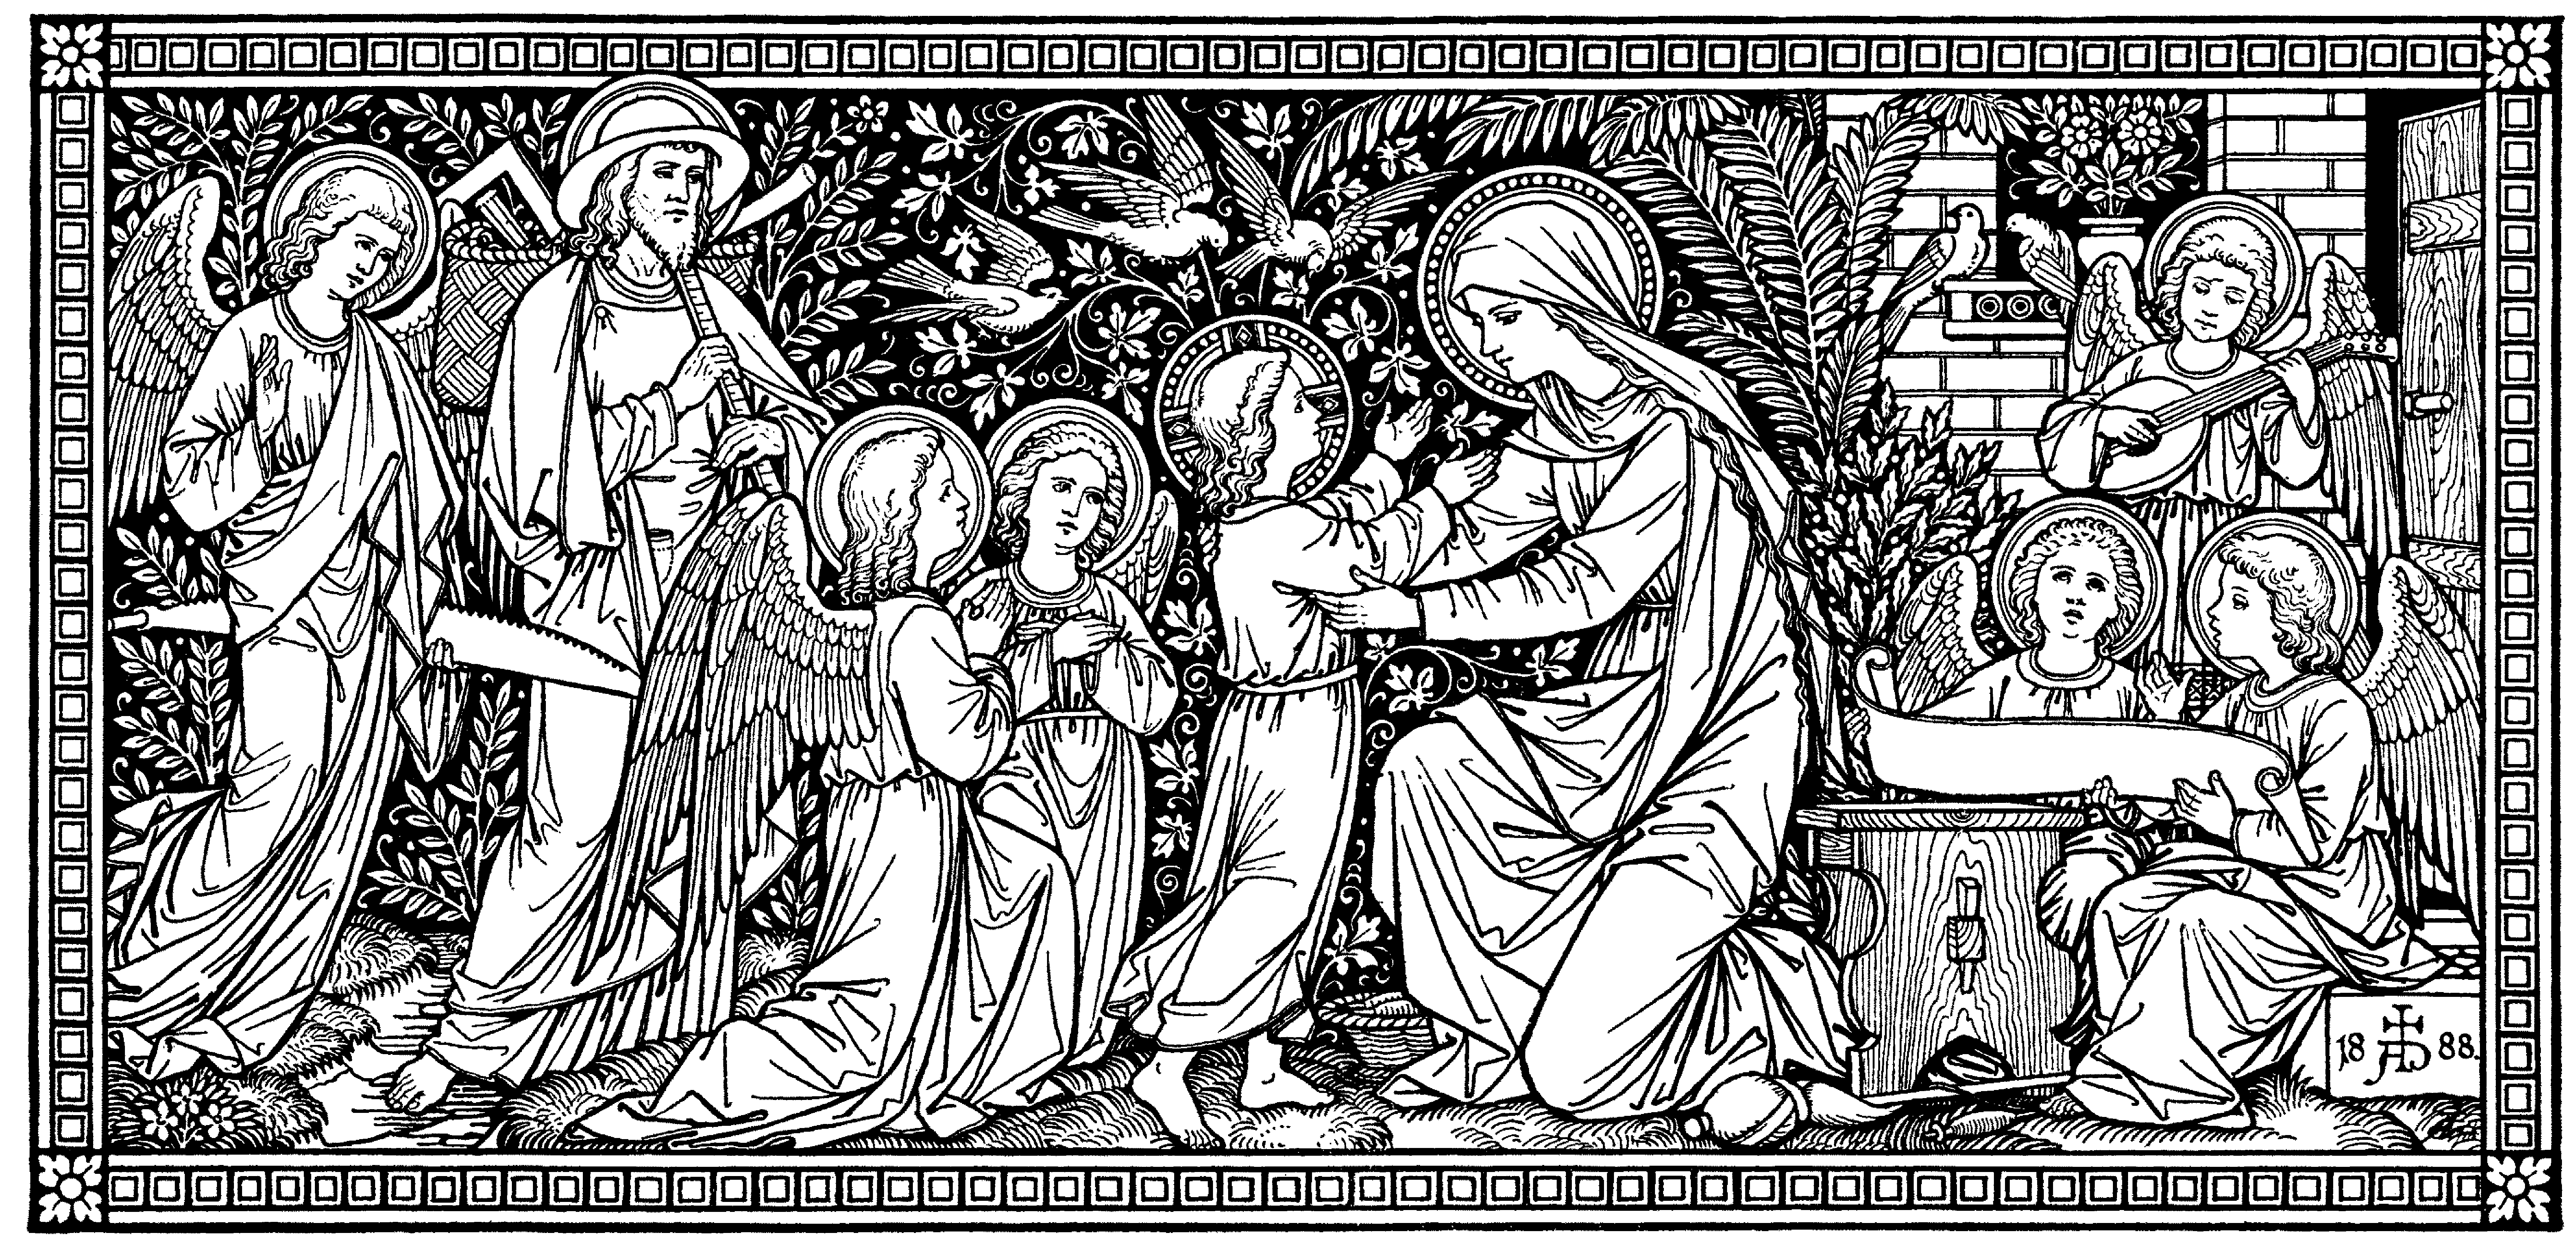
\includegraphics[height=5.5cm]{images/SainteFamille}
%\end{center}





\end{document}